\documentclass{classrep}
\usepackage[utf8]{inputenc}
\usepackage{color}
\usepackage{graphicx} 
\DeclareUnicodeCharacter{00A0}{~}

\studycycle{Informatyka, studia dzienne, inż I st.}
\coursesemester{IV}

\coursename{Sztuczna inteligencja i systemy ekspertowe}
\courseyear{2021/2022}

\courseteacher{dr inż. Krzysztof Lichy}
\coursegroup{poniedziałek, 12:00}

\author{
  \studentinfo{Trung Anh Nguyen Nang}{236613} \and
  \studentinfo{Tomasz Makowski}{236593}
}

\title{Zadanie 2: Mapowanie lokalizacji na siatkę}

\begin{document}
\maketitle



\section{Cel}
{Celem jest łatwe i szybkie sprawdzenie obecności na zajęciach.}

\section{Wprowadzenie}
{Do naszej aplikacji wykorzystujemy HTML, oraz język JavaScript a w nim wykorzystujemy globalny obiekt navigator. Co więcej wykorzystujemy biblioteke Leaflet.js która dostarcza nam mape świata w raz z możliwością jej obsługi.}

\section{Opis implementacji}
{Nasza aplikacja składa się z 2 częsci.Pierwsza część logiczna jest napisana w JavaScript, a druga jest w HTML. W części logicznej znajduję się jedna rozbudowana klasa.
Ta klasa ma za zadanie: 
\begin{itemize}
\item inicjalizuje naszą mape
\item odświeża nasze aktualne położenie co sekunde
\item dodaje oraz obsługuje mape CTI
\item pokazuje oraz wypisuje w jakim pokoju w CTI aktualnie się znajdujesz
\item sprawdza też czy wgl jesteś w CTI
\end{itemize}}

\section{Materiały i metody}
{Wszystkie nasze badania opierały się o testowanie jakości i dokładności GPS w telefonie oraz jak sobie on radzi w miejscach ze słabym zasięgiem.Aby to zrobić uruchomiliśmy naszą gotową aplikacje w przeglądarce na telefonie komórkowym. Dalszym krokiem było udanie się do budynku CTI i tam przetestowanie jakości dostarczanych danych przez GPS w zależności od naszego położenia}

\section{Wyniki}
{
\begin{figure}[ht]

    \centering

  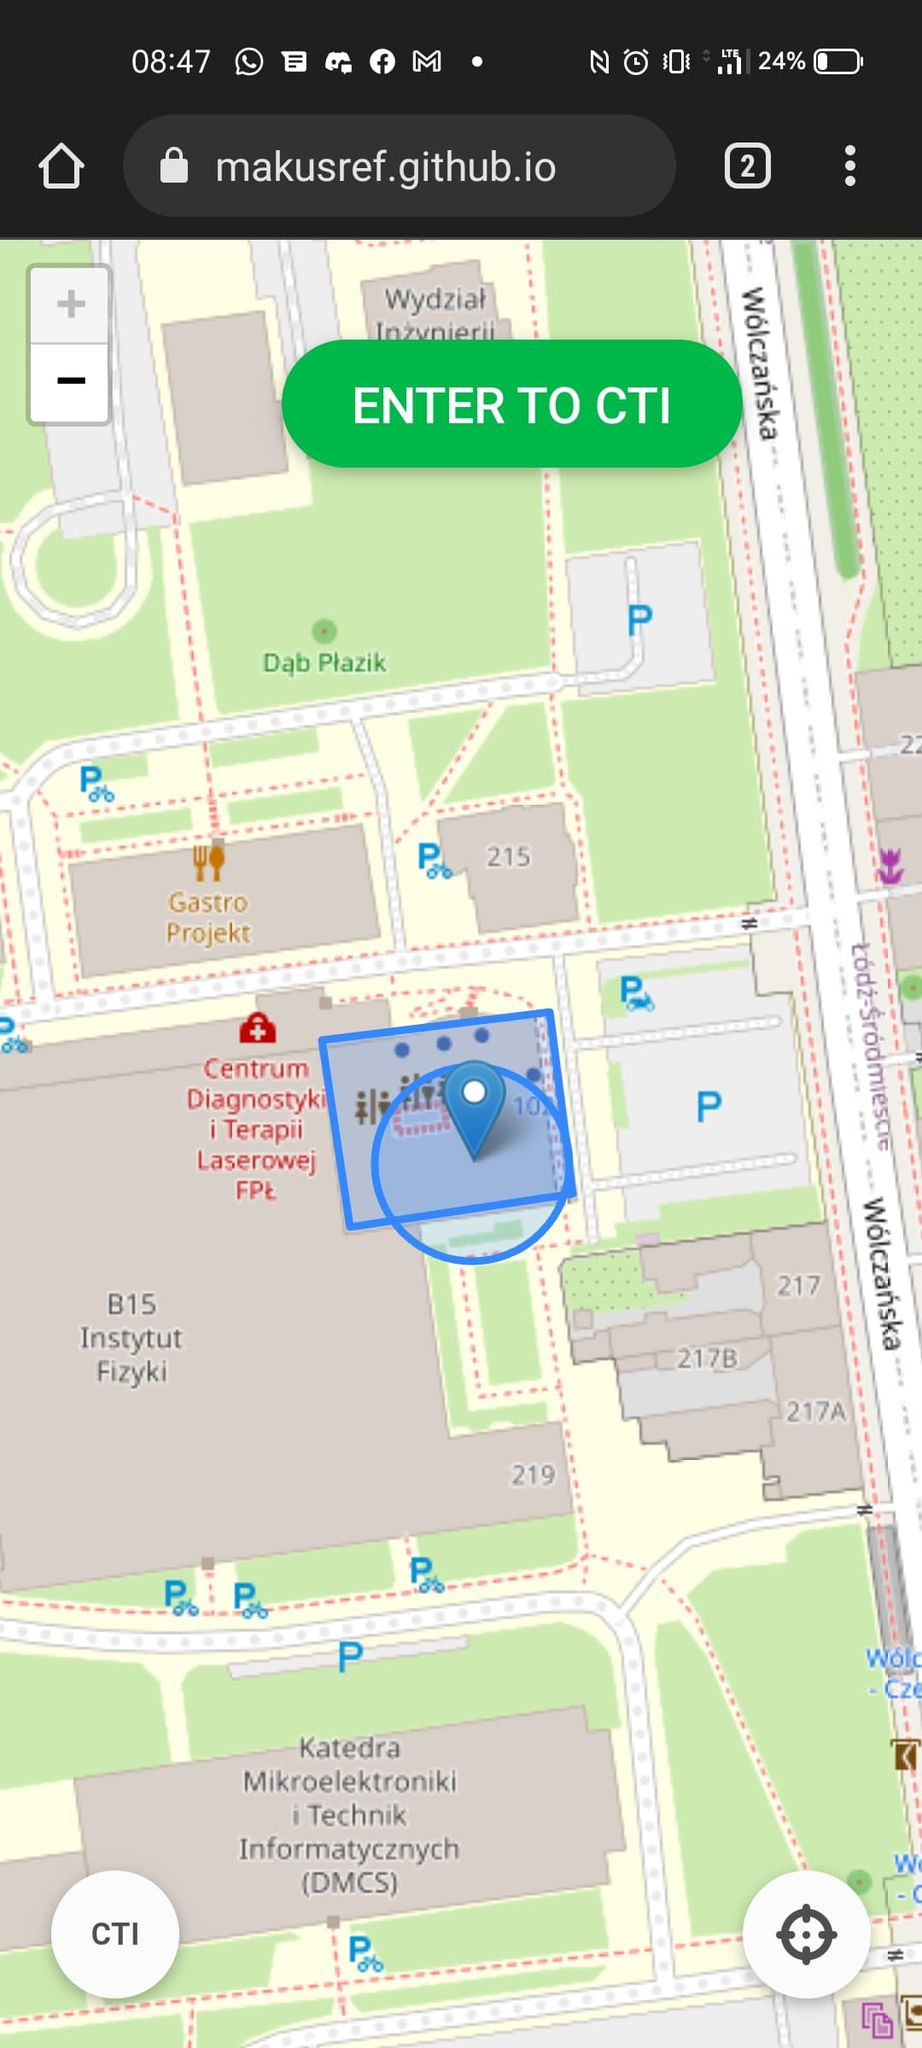
\includegraphics[scale=0.2]{photo1.png}

    \caption{Początek aplikacji}

    \label{fig}

\end{figure}
\begin{figure}[ht]

    \centering

  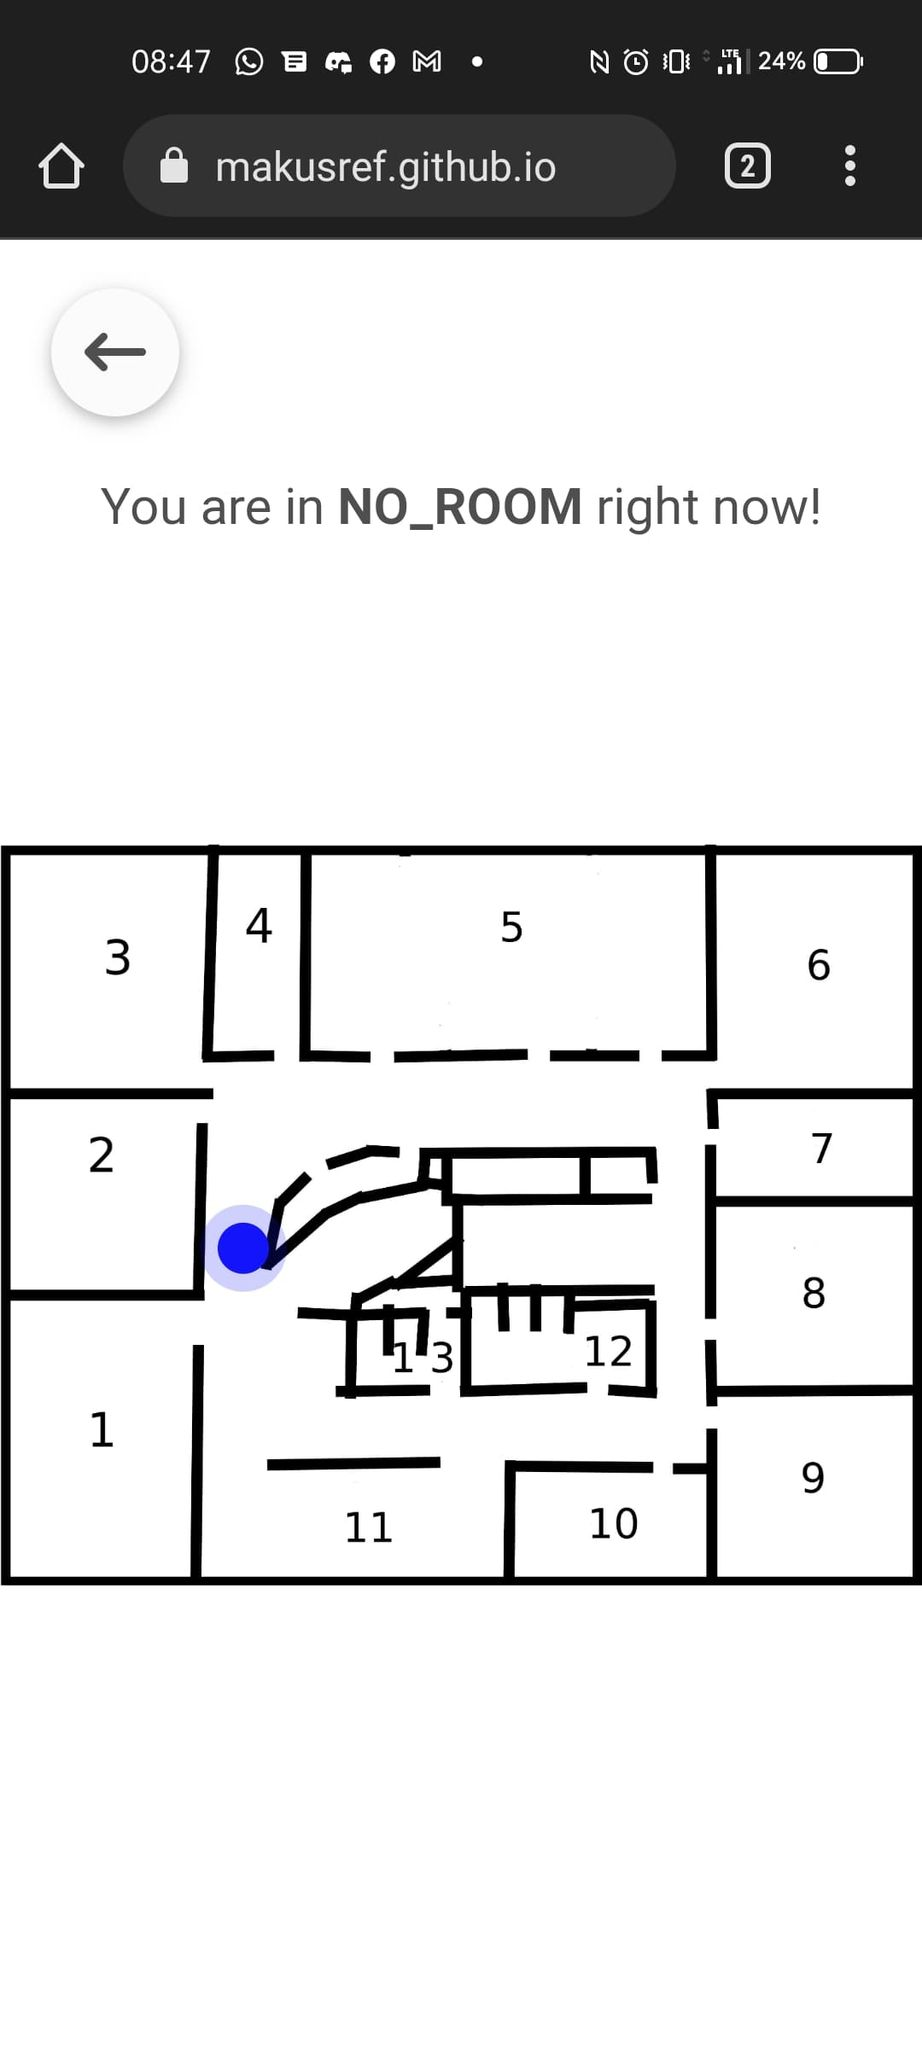
\includegraphics[scale=0.2]{photo2.png}

    \caption{Mapa CTI}

    \label{fig}

\end{figure}
}

\section{Dyskusja}
{Gdy użytkownik jest przy jakieś ścianie, program może nie wskazać dość precyzyjnie jakbyśmy chcieli. Spodowodowane to jest wymiar naszej mapy,który ustawialiśmy odległości między ścianami ludzkim okiem mniej więcej. Dodatkowy powód jest nierówny rysunek , co nieodzwierciedla kształtów budynków w 100 procentach.Dużym problemem też jest odwrócona mapa, co utrudnia stwierdzenie poprawności działania programu.}

\section{Wnioski}
{Aplikacje całkiem dobrze wskazuje lokalizacje. Mniej więcej w szybki i prosty sposób wskazuje położenie osoby, która korzysta z aplikacji.}

\begin{thebibliography}
{1}\bibitem{http} \url{https://developer.mozilla.org/pl/docs/Web/API/Geolocation_API}
{2}\bibitem{http} \url{https://leafletjs.com/index.html#map-example}
\end{thebibliography}


\end{document}
